\chapter{Конструкторский раздел}

\section{Проектируемая база данных}

На рисунке~\ref{fig:uml} представлена диаграмма проектируемой базы данных.
\begin{figure}[h]
    \centering
    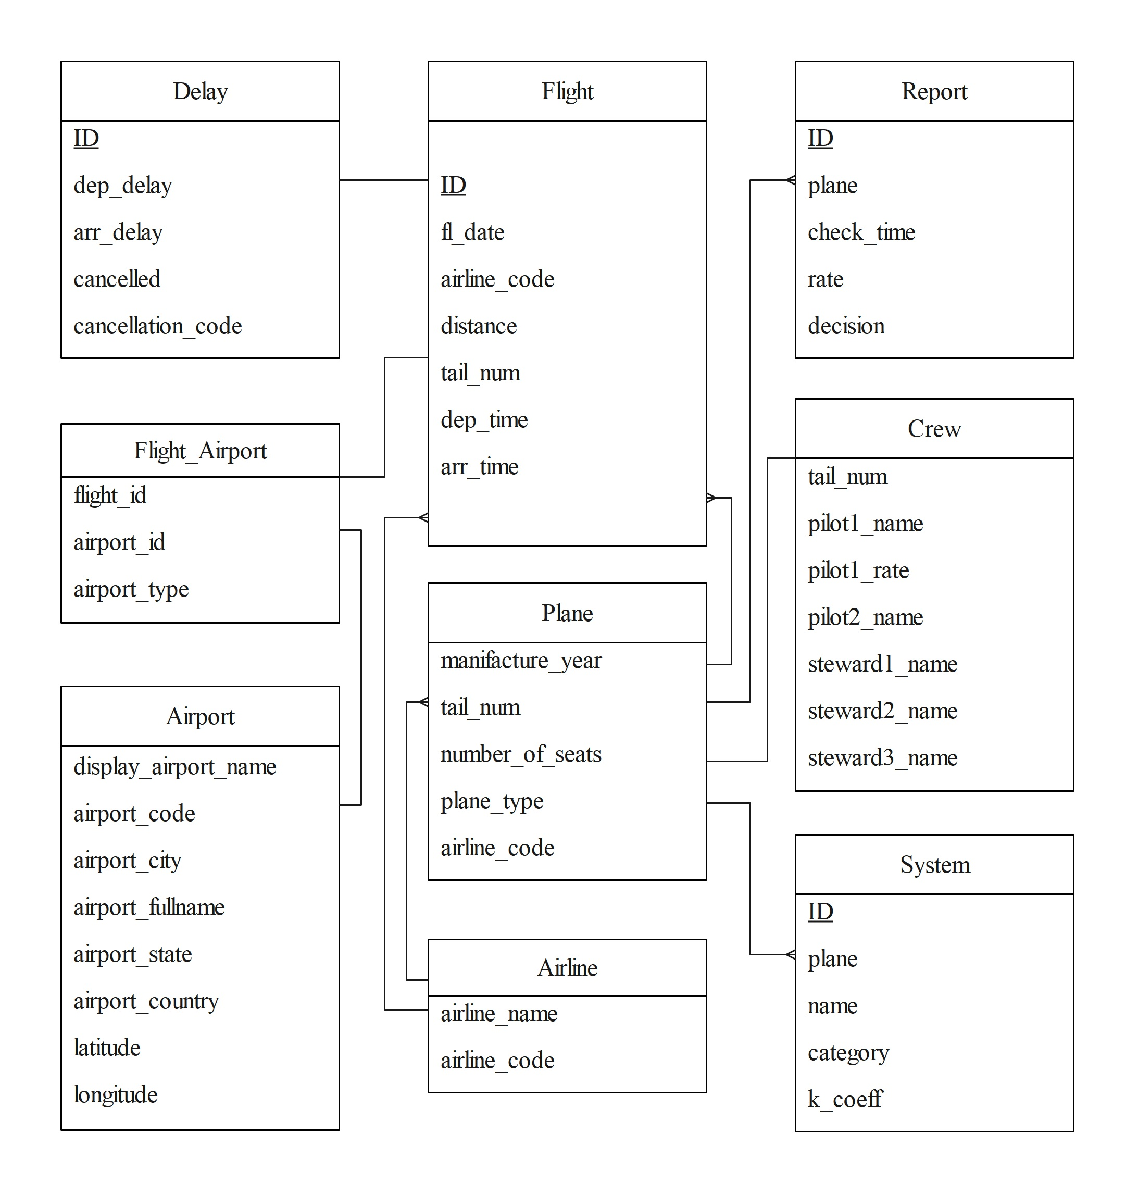
\includegraphics[scale=0.9]{inc/Drawing3}
    \caption{Диаграмма проектируемой базы данных}
    \label{fig:uml}
\end{figure}

\newpage
В таблицах~\ref{tab:tabl1}--~\ref{tab:tabl9} представлены описания полей соответствующих таблиц базы данных:

\begin{table}[H]
    \centering
    \captionsetup{justification=centering}
    \caption{Описание таблицы flight}
    \begin{tabular}{|p{0.4\textwidth}|p{0.4\textwidth}|}
        \hline
        Атрибут & Тип данных \\
        \hline
        Идентификатор & Целое число \\
        Дата вылета & Дата \\
        Код авиакомпании & Строка \\
        Время вылета & Время \\
        Время прилета & Время \\
        Длина пути (в милях) & Вещественное число \\
        Время в пути & Вещественное число \\
        Номер борта & Строка \\
        \hline
    \end{tabular}
    \label{tab:tabl1}
\end{table}

\begin{table}[H]
    \centering
    \captionsetup{justification=centering}
    \caption{Описание таблицы delay}
    \begin{tabular}{|p{0.4\textwidth}|p{0.4\textwidth}|}
        \hline
        Атрибут & Тип данных \\
        \hline
        Идентификатор & Целое число \\
        Задержка вылета & Вещественное число \\
        Задержка прилета & Вещественное число \\
        Статус & Целое число \\
        Причина отмены & Строка \\
        \hline
    \end{tabular}
    \label{tab:tabl2}
\end{table}

\begin{table}[H]
    \centering
    \captionsetup{justification=centering}
    \caption{Описание таблицы airport}
    \begin{tabular}{|p{0.4\textwidth}|p{0.4\textwidth}|}
        \hline
        Атрибут & Тип данных \\
        \hline
        Название & Строка \\
        Код аэропорта & Строка \\
        Город & Строка \\
        Полное имя & Строка \\
        Страна & Строка \\
        Географская ширина & Вещественное число \\
        Географская высота & Вещественное число \\
        \hline
    \end{tabular}
    \label{tab:tabl3}
\end{table}

\begin{table}[H]
    \centering
    \captionsetup{justification=centering}
    \caption{Описание таблицы airline}
    \begin{tabular}{|p{0.4\textwidth}|p{0.4\textwidth}|}
        \hline
        Атрибут & Тип данных \\
        \hline
        Название & Строка \\
        Код авиакомпании & Строка \\
        \hline
    \end{tabular}
    \label{tab:tabl4}
\end{table}

\begin{table}[H]
    \centering
    \captionsetup{justification=centering}
    \caption{Описание таблицы plane}
    \begin{tabular}{|p{0.4\textwidth}|p{0.4\textwidth}|}
        \hline
        Атрибут & Тип данных \\
        \hline
        Год выпуска & Целое число \\
        Номер борта & Строка \\
        Количество мест & Целое число \\
        Модель & Строка \\
        Код авиакомпании & Строка \\
        \hline
    \end{tabular}
    \label{tab:tabl5}
\end{table}

\begin{table}[H]
    \centering
    \captionsetup{justification=centering}
    \caption{Описание таблицы crew}
    \begin{tabular}{|p{0.4\textwidth}|p{0.4\textwidth}|}
        \hline
        Атрибут & Тип данных \\
        \hline
        Номер борта & Строка \\
        ФИО первого пилота & Строка \\
        ФИО второго пилота & Строка \\
        ФИО первого стююарда & Строка \\
        ФИО второго стьюарда & Строка \\
        ФИО третьего стьюарда & Строка \\
        \hline
    \end{tabular}
    \label{tab:tabl6}
\end{table}

\begin{table}[H]
    \centering
    \captionsetup{justification=centering}
    \caption{Описание таблицы report}
    \begin{tabular}{|p{0.4\textwidth}|p{0.4\textwidth}|}
        \hline
        Атрибут & Тип данных \\
        \hline
        Идентификатор & Целое число \\
        Номер борта & Строка \\
        Время создания отчета & Время \\
        Оценка & Вещественное число \\
        Решение & Логический тип \\
        \hline
    \end{tabular}
    \label{tab:tabl7}
\end{table}

\begin{table}[H]
    \centering
    \captionsetup{justification=centering}
    \caption{Описание таблицы system}
    \begin{tabular}{|p{0.4\textwidth}|p{0.4\textwidth}|}
        \hline
        Атрибут & Тип данных \\
        \hline
        Идентификатор & Целое число \\
        Номер борта & Строка \\
        Имя & Строка \\
        Категория & Строка \\
        Коэффициент износа & Вещественное число \\
        \hline
    \end{tabular}
    \label{tab:tabl8}
\end{table}

\begin{table}[H]
    \centering
    \captionsetup{justification=centering}
    \caption{Описание таблицы flight\_airport}
    \begin{tabular}{|p{0.4\textwidth}|p{0.4\textwidth}|}
        \hline
        Атрибут & Тип данных \\
        \hline
        Идентификатор полета & Целое число \\
        Идентификатор аэропорта & Целое число \\
        Тип аэропорта & Строка \\
        \hline
    \end{tabular}
    \label{tab:tabl9}
\end{table}

\section{Описание используемого триггера}

Для автоматического обновления данных в таблице system при добавлении нового отчета о самолете в таблицу report был создан триггер, который автоматически обновляет поле k\_coeff всех систем таблицы system, которые относятся к самолету.

На рисунке~\ref{fig:trigger} изображена схема алгоритма функции триггера.

\begin{figure}[H]
    \centering
    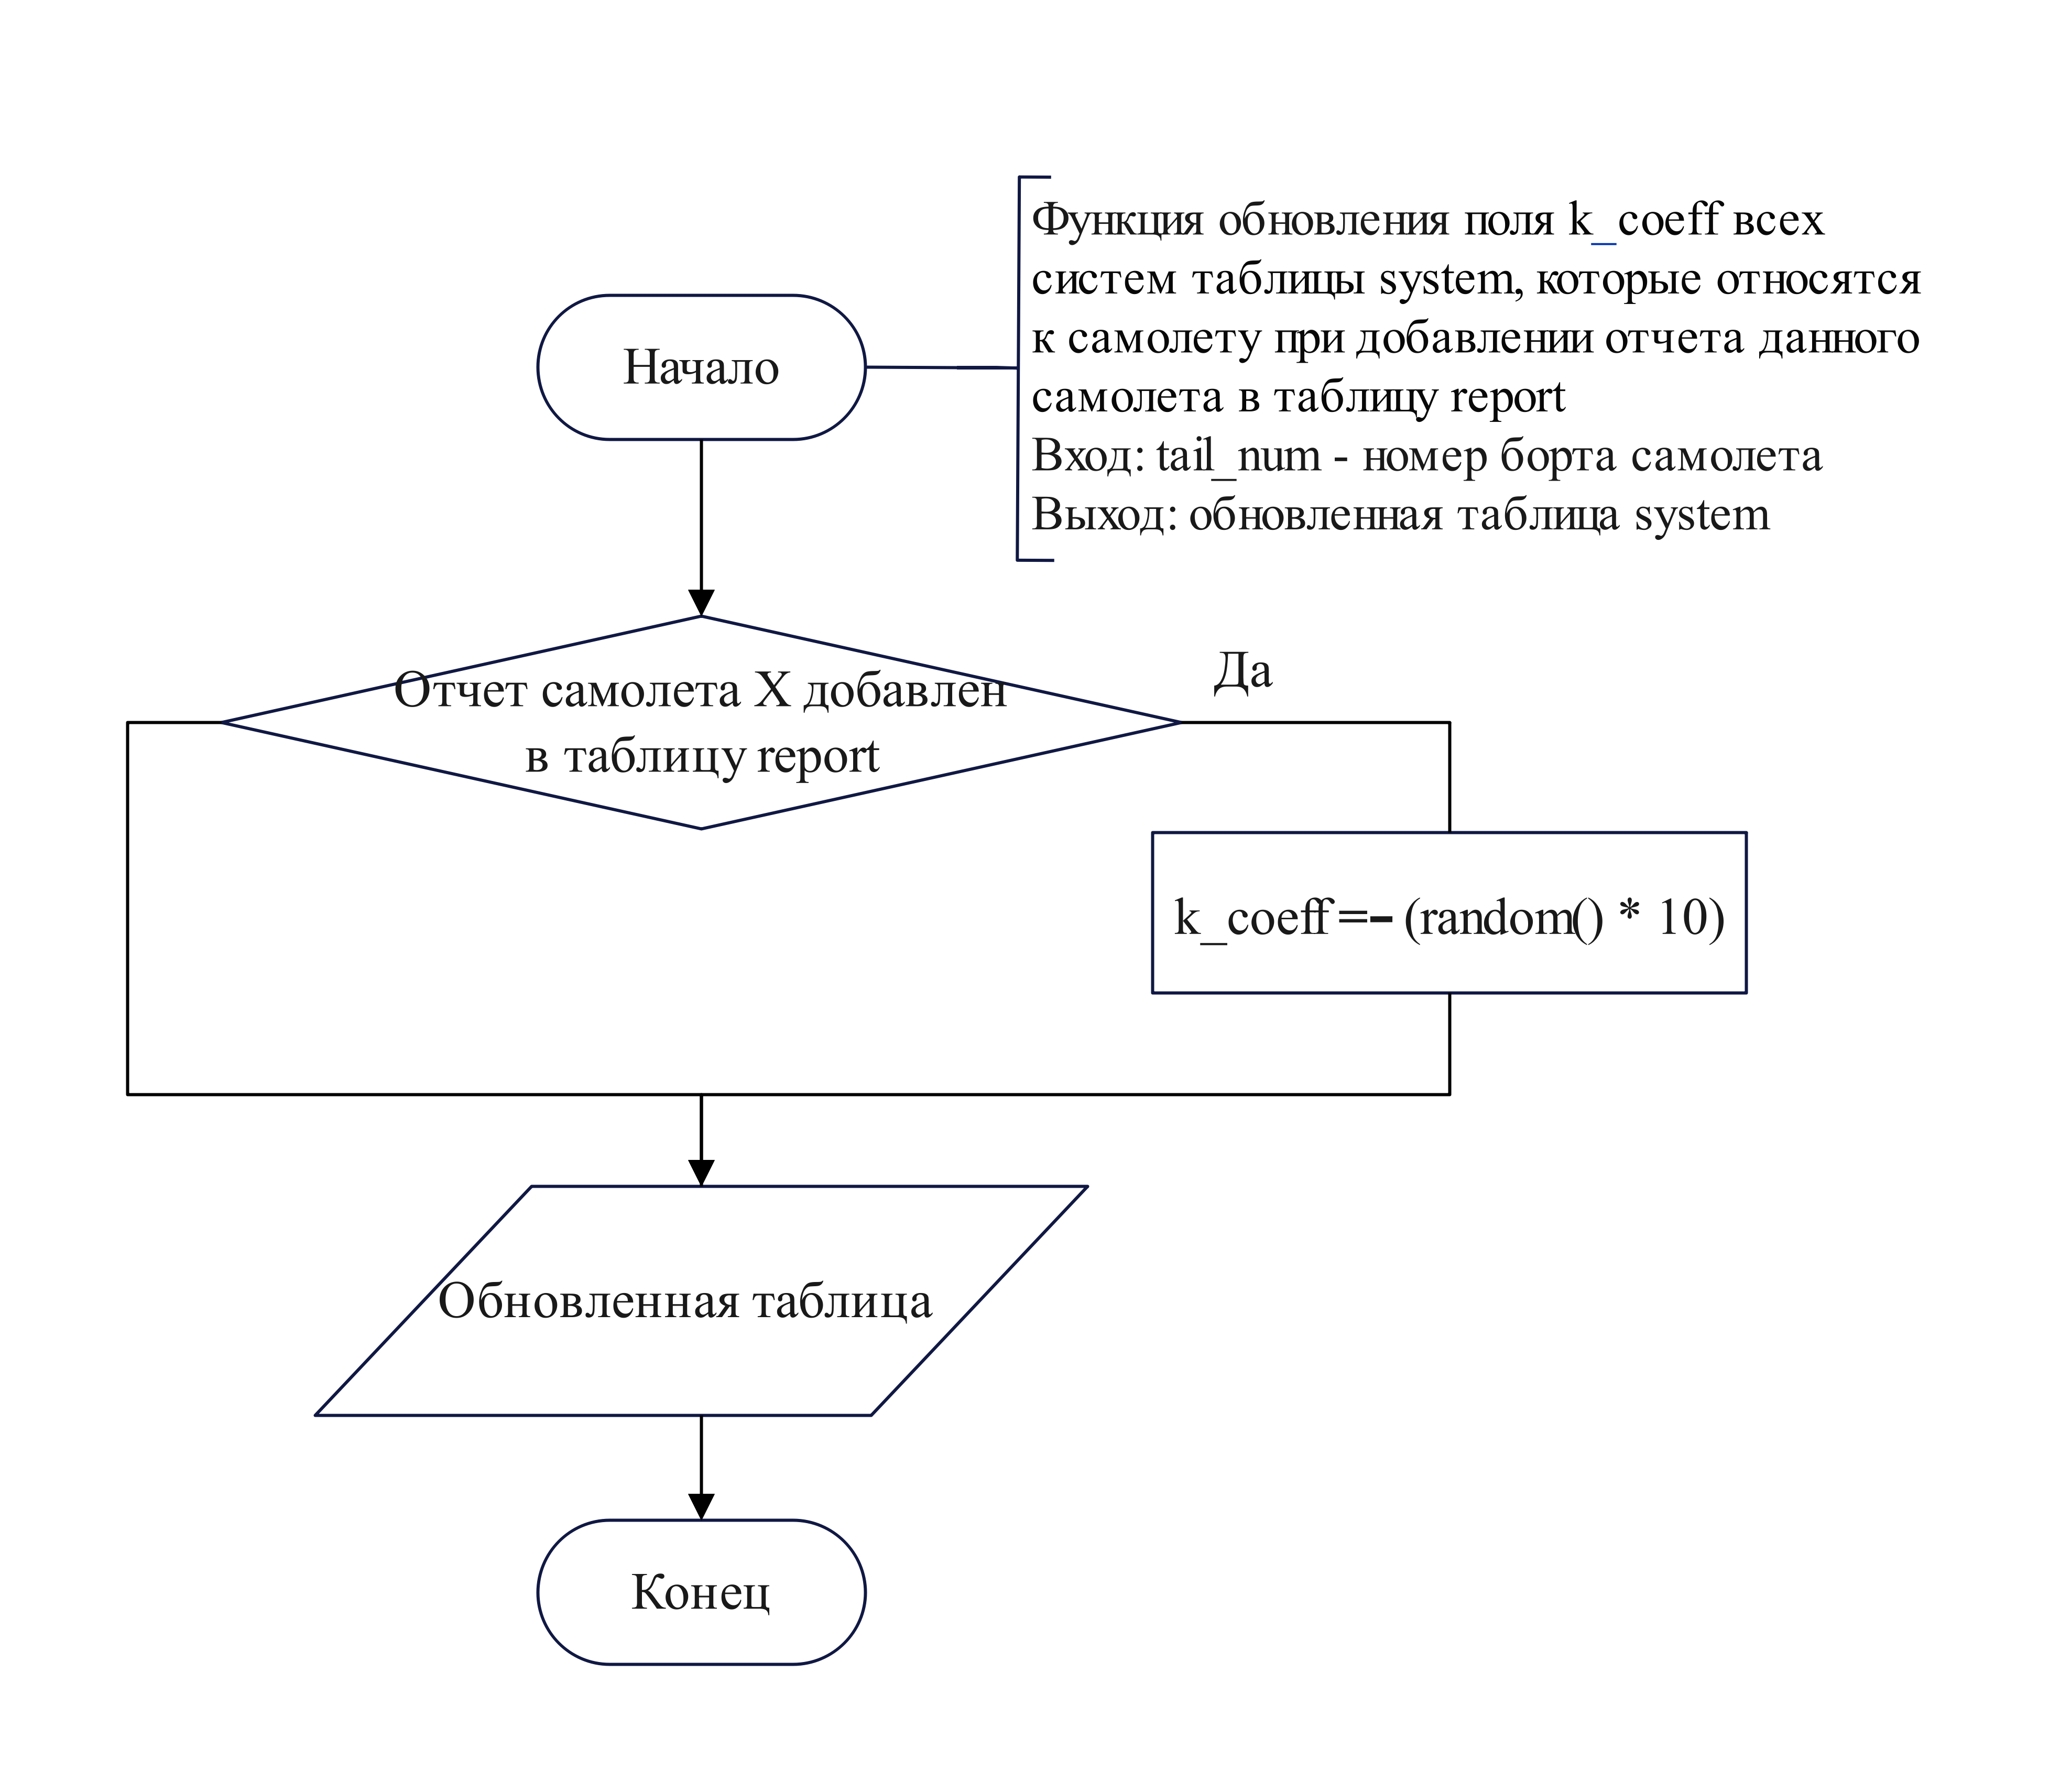
\includegraphics[scale=0.8]{inc/Drawing4}
    \caption{Схема алгоритма функции триггера}
    \label{fig:trigger}
\end{figure}

\section{Описание используемой хранимой процедуры}

Для получения информации о вероятности задержки рейса была создана хранимая процедура, которая принимает на вход идентификаторы полета, аэропортов взлета и посадки, а также дату, до которой производится перебор всех полетов для вычисления вероятности задержки.

На рисунке~\ref{fig:procedure} изображена схема алгоритма хранимой процедуры.

\begin{figure}[H]
    \centering
    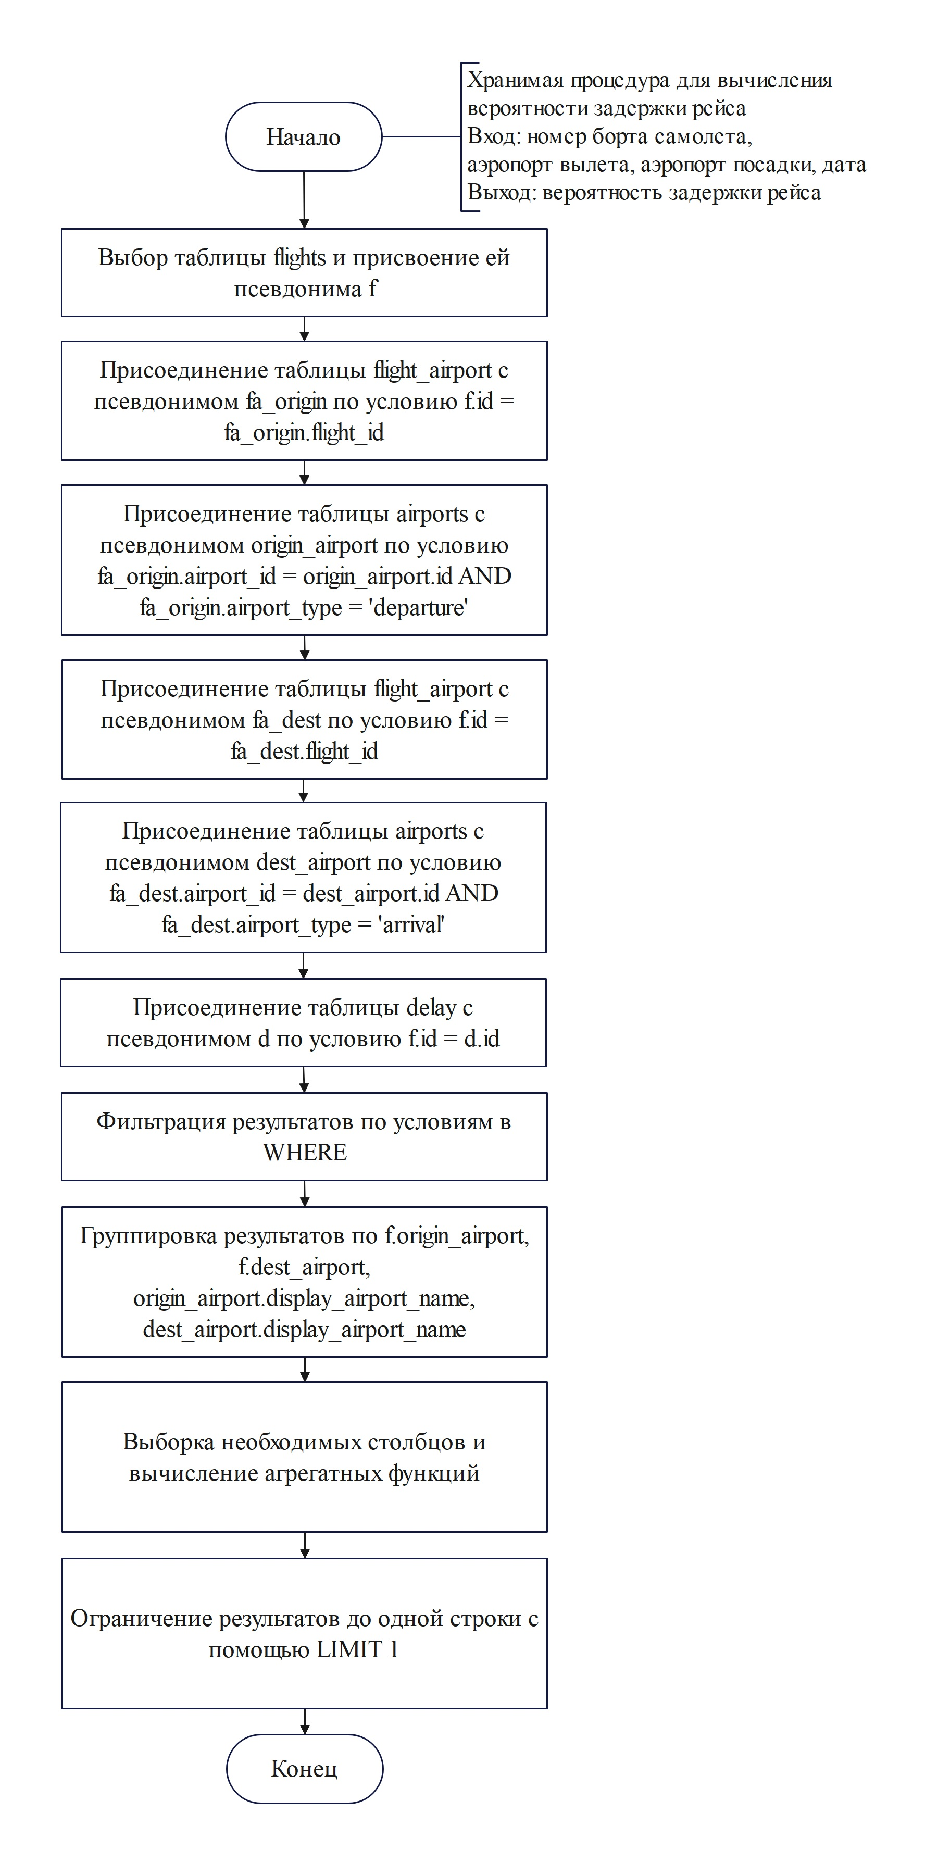
\includegraphics[scale=0.8]{inc/Drawing5}
    \caption{Схема алгоритма хранимой процедуры}
    \label{fig:procedure}
\end{figure}

Для вычисления вероятности задержки рейса была использована формула:
\begin{equation}
    P = \frac{N_{\text{задержанных}}}{N_{\text{всех}}}, \label{eq:prob}
\end{equation}
где $N_{\text{задержанных}}$ --- количество задержанных рейсов, $N_{\text{всех}}$ --- общее количество рейсов.

Вероятность задержки рассчитывается как отношение количества задержанных рейсов к общему числу рейсов для конкретного самолета, места взлета и посадки до указанной даты.

\section{Система ролей в базе данных}

В контексте разработанной базы данных были определены три основные роли: гость, сотрудник и администратор.
Эти роли были созданы для обеспечения разграничения доступа к данным и функциональности базы данных.

\begin{enumerate}[label=---]
    \item Роль ``Гость'' предоставляет возможность просмотра информации о полетах, аэропортах, авиакомпаниях и задержках, а также может получить информацию о вероятности задержки конкретного перелета.
    Это обеспечивает доступ к общедоступной информации без возможности ее изменения.
    \item Роль ``Сотрудник'' предоставляет возможность просмотра, добавления или изменения информации о системах самолетов и отчетах.
    Это позволяет сотрудникам обновлять и поддерживать актуальность данных, необходимых для их работы, при этом ограничивая их доступ только к определенным частям базы данных.
    \item Роль '`Администратор'' предоставляет полный доступ к функциональности базы данных, включая просмотр, добавление или изменение информации о полетах, аэропортах, авиакомпаниях, самолетах, задержках, экипаже, системах самолетов и отчетах.
    Администратор также может получить информацию о вероятности задержки конкретного перелета.
\end{enumerate}

Система ролей является важным элементом обеспечения безопасности и целостности данных.
Она позволяет контролировать доступ к данным и предотвращает несанкционированные изменения или удаление информации.

